% SC3270 --- Chapter 8: Refinement and Correctness by Construction (0->100 ground-up)
\chapter{Refinement and Correctness by Construction}
\label{ch:refinement}

\begin{quote}
\emph{``Do not verify after the fact; construct so that correctness is the only outcome.''} Refinement turns a specification into code by small, proved steps—like carving a statue by successive, measured cuts.
\end{quote}

\noindent\fbox{\parbox{\dimexpr\linewidth-2\fboxsep-2\fboxrule}{%
\textbf{From zero: no refinement background assumed.} We define refinement from specifications to programs, present Morgan's laws, and build two programs—binary search and list reversal—by calculation, not guess-and-verify. Only Hoare triples and invariants are assumed.}}
\vspace{0.4em}

\section*{Learning Outcomes}
After this chapter you will be able to:
\begin{enumerate}[label=(L\arabic*)]
    \item define refinement $S \sqsubseteq C$ and its relation to Hoare triples;
    \item apply refinement laws for composition, conditional, and loop introduction;
    \item derive a loop from a spec via invariant and variant as construction steps;
    \item contrast post-hoc verification with correctness by construction;
    \item sketch a refinement chain from abstract spec to executable heap code.
\end{enumerate}

% ============================================================
\section{From Post-Hoc Proof to Construction}
\label{sec:post-hoc-vs-calc}
\paragraph{Intuition.} Post-hoc verification writes code first, then tries to prove $\{P\}\,C\,\{Q\}$. When the proof fails you patch code and retry—a costly loop. Correctness by construction inverts the flow: start from the spec $S\equiv\{P\}\,?\,\{Q\}$ (a hole where code will go) and \emph{refine} it stepwise, each step preserving correctness. When the hole is filled, no separate proof is needed—the construction \emph{is} the proof.

\begin{definition}[Specification statement and refinement]
Write $x:[P,Q]$ for ``change only $x$ to establish $Q$, assuming $P$''. More generally $w:[P,Q]$ where $w$ is the frame (variables allowed to change). Then $S \sqsubseteq C$ (``$C$ refines $S$'') iff for all $P,Q$ with $\{P\}\,S\,\{Q\}$, also $\{P\}\,C\,\{Q\}$—every spec satisfied by $S$ is satisfied by $C$. In Hoare terms, $w:[P,Q] \sqsubseteq C$ iff $\{P\}\,C\,\{Q\}$ and $C$ modifies only $w$.
\end{definition}

\begin{figure}[h]\centering
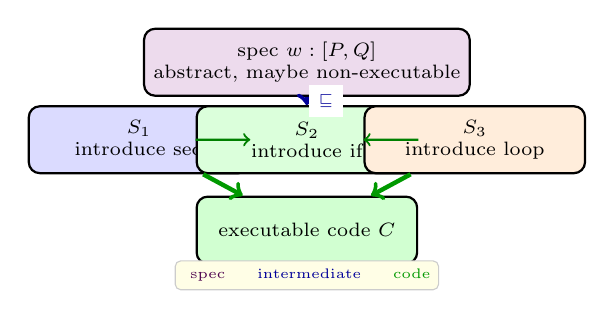
\begin{tikzpicture}[scale=0.82,font=\scriptsize,
  box/.style={draw,thick,rounded corners=4pt,align=center,minimum width=2.8cm,minimum height=0.85cm}]
\node[box,fill=violet!14] (spec) at (4.2,2.6) {spec $w:[P,Q]$\\abstract, maybe non-executable};
\node[box,fill=blue!14] (step1) at (1.6,1.4) {$S_1$\\introduce seq};
\node[box,fill=green!14] (step2) at (4.2,1.4) {$S_2$\\introduce if};
\node[box,fill=orange!14] (step3) at (6.8,1.4) {$S_3$\\introduce loop};
\node[box,fill=green!18] (code) at (4.2,0.0) {executable code $C$};
\draw[->,ultra thick,blue!60!black] (spec) -- (step2) node[midway,right,font=\tiny,fill=white] {$\sqsubseteq$};
\draw[->,thick,green!50!black] (step2) -- (step1);
\draw[->,thick,green!50!black] (step2) -- (step3);
\draw[->,ultra thick,green!60!black] (step1) -- (code);
\draw[->,ultra thick,green!60!black] (step3) -- (code);
\node[font=\tiny,align=left,fill=yellow!10,draw=gray!40,rounded corners=2pt,inner sep=3pt] at (4.2,-0.70) {\textcolor{violet!60!black}{$\blacksquare$ spec} \quad \textcolor{blue!60!black}{$\blacksquare$ intermediate} \quad \textcolor{green!60!black}{$\blacksquare$ code}};
\end{tikzpicture}
\caption{Refinement lattice: start at spec (top, violet), descend by law-driven steps to code (bottom, green). Each arrow $\sqsubseteq$ is a proved law, so correctness flows downward.}
\label{fig:refinement-lattice}
\end{figure}

\begin{figure}[h]\centering
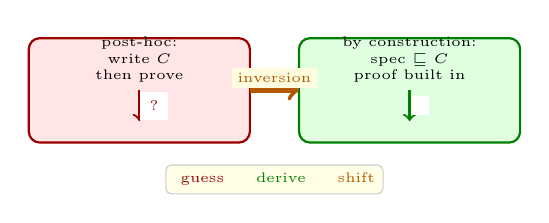
\begin{tikzpicture}[scale=0.78,font=\scriptsize]
\draw[fill=red!10,draw=red!60!black,thick,rounded corners=4pt] (0,0) rectangle (3.6,1.70);
\node[font=\tiny,align=center] at (1.80,1.35) {post-hoc:\\ write $C$\\then prove};
\draw[->,thick,red!60!black] (1.80,0.85) -- (1.80,0.35) node[midway,right,font=\tiny,fill=white] {?};
\draw[fill=green!12,draw=green!50!black,thick,rounded corners=4pt] (4.4,0) rectangle (8.0,1.70);
\node[font=\tiny,align=center] at (6.20,1.35) {by construction:\\ spec $\sqsubseteq$ $C$\\ proof built in};
\draw[->,thick,green!50!black] (6.20,0.85) -- (6.20,0.35) node[midway,right,font=\tiny,fill=white] {$\checkmark$};
\draw[->,ultra thick,orange!70!black] (3.6,0.85) -- (4.4,0.85) node[midway,above,font=\tiny,fill=yellow!12,inner sep=2pt] {inversion};
\node[font=\tiny,align=left,fill=yellow!10,draw=gray!40,rounded corners=2pt,inner sep=3pt] at (4.0,-0.60) {\textcolor{red!60!black}{$\blacksquare$ guess} \quad \textcolor{green!50!black}{$\blacksquare$ derive} \quad \textcolor{orange!70!black}{$\blacksquare$ shift}};
\end{tikzpicture}
\caption{Two workflows: post-hoc guesses code then struggles to prove; construction derives code from spec so the proof is intrinsic. The arrow is inverted.}
\label{fig:posthoc-vs-construct}
\end{figure}

% ============================================================
\section{Laws of Refinement}
\label{sec:laws}
Each law is an equivalence justified by Hoare logic. Core laws (Morgan):

\textbf{Skip:} $w:[P,P]\sqsubseteq \texttt{skip}$.

\textbf{Assignment:} $x:[P, Q[x\mapsto e]] \sqsubseteq x:=e$ when $x\in w$.

\textbf{Sequence:} $w:[P,R]\sqsubseteq w:[P,Q];\,w:[Q,R]$ (introduce intermediate $Q$).

\textbf{Conditional:} $w:[P,Q]\sqsubseteq \texttt{if }B\texttt{ then }w:[P\land B,Q]\texttt{ else }w:[P\land\neg B,Q]$.

\textbf{Loop (with invariant $I$ and variant $V$):} $w:[I,\;I\land\neg B]\sqsubseteq \texttt{while }B\texttt{ do }w:[I\land B,\;I\land V<v_0]$ where $v_0$ is logical snapshot of $V$ on entry.

Each law's side conditions are VCs; discharging them guarantees the step is sound. So refinement is Hoare logic turned into a \emph{design} calculus.

\begin{example}[Conditional refinement]
Spec to compute $m=\max(a,b)$: $m:[ \text{true},\; m\ge a\land m\ge b\land(m=a\lor m=b)]$. By conditional law with $B\equiv a\ge b$, refine to $\texttt{if }a\ge b\texttt{ then }m:[a\ge b,\;m=a]\texttt{ else }m:[a<b,\;m=b]$, then each branch refines by assignment $m:=a$ and $m:=b$ respectively. The $B$ case split was forced by the spec's disjunction.
\end{example}

\begin{remark}[Data refinement]
Beyond code, you refine \emph{data}: abstract set $S$ to concrete array $a$ with coupling invariant $S=\{a[i]:0\le i<n\}$. Operations on $S$ (add, member) refine to array manipulations that preserve the coupling. This is how abstract specs of collections become efficient implementations without breaking proved properties.
\end{remark}

\begin{lstlisting}[language=Java, caption={Specification statement as JML contract: the abstract spec to be refined.}, label={lst:spec-java}]
/* @ requires n >= 0 && sorted(a,0,n-1);
  @ ensures (\result==-1 ==> forall k. a[k]!=key) &&
  @         (\result>=0 ==> a[\result]==key);
  @ assignable \nothing; // abstract spec, no code yet
  @*/
// w:[P,Q] where w={result}, P=sorted&&n>=0, Q=found-or-not
int spec_search(int[] a,int n,int key);
\end{lstlisting}

% ============================================================
\section{Construction in Action: Binary Search}
\label{sec:binary-search}
Spec: $r:[ \text{sorted}(a[0..n))\land0\le n,\; (r\ge0\Rightarrow a[r]=key)\land(r=-1\Rightarrow key\notin a)]$.

Step 1---introduce variables $lo,hi$ and strengthen invariant:
\[
I\equiv 0\le lo\le hi\le n\land (\forall i<lo.\,a[i]<key)\land(\forall i\ge hi.\,a[i]>key)
\]
with $lo:=0;hi:=n$ establishing $I$ (VC: $P\Rightarrow I[lo,hi\mapsto0,n]$).

Step 2---loop \texttt{while $lo<hi$ do } with variant $V\equiv hi-lo$. Introduce mid $m:=(lo+hi)/2$ inside, then conditional on $a[m]$ vs.\ $key$: if $a[m]<key$ then $lo:=m+1$ else if $a[m]>key$ then $hi:=m$ else $r:=m;\,lo:=hi$ (found). Each branch preserves $I$ and decreases $V$ (gap shrinks by at least half). Exit $lo=hi$ gives $I\land lo=hi\land\neg(lo<hi)$ plus the two quantified halves imply $key$ absent, so $r:=-1$ establishes $Q$.

Calculation produced the classic binary search without ever running a test—the invariant dictated every branch.

\begin{figure}[h]\centering
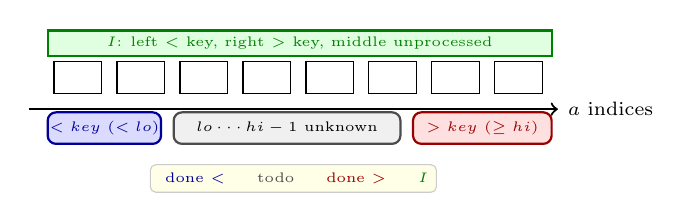
\begin{tikzpicture}[scale=0.80,font=\scriptsize]
\draw[->,thick] (0,0) -- (8.4,0) node[right] {$a$ indices};
\foreach \x in {0.4,1.4,2.4,3.4,4.4,5.4,6.4,7.4} \draw (\x,0.25) rectangle (\x+0.75,0.75);
\draw[fill=blue!14,draw=blue!60!black,thick,rounded corners=3pt] (0.30,-0.55) rectangle (2.10,-0.05);
\node[font=\tiny,blue!60!black] at (1.20,-0.30) {$<key$ ($<lo$)};
\draw[fill=gray!12,draw=gray!60!black,thick,rounded corners=3pt] (2.30,-0.55) rectangle (5.90,-0.05);
\node[font=\tiny] at (4.10,-0.30) {$lo \cdots hi-1$ unknown};
\draw[fill=red!12,draw=red!60!black,thick,rounded corners=3pt] (6.10,-0.55) rectangle (8.30,-0.05);
\node[font=\tiny,red!60!black] at (7.20,-0.30) {$>key$ ($\ge hi$)};
\draw[fill=green!12,draw=green!50!black,thick] (0.30,0.85) rectangle (8.30,1.25);
\node[font=\tiny,green!50!black] at (4.30,1.05) {$I$: left $<$ key, right $>$ key, middle unprocessed};
\node[font=\tiny,align=left,fill=yellow!10,draw=gray!40,rounded corners=2pt,inner sep=3pt] at (4.2,-1.10) {\textcolor{blue!60!black}{$\blacksquare$ done $<$} \quad \textcolor{gray!60!black}{$\blacksquare$ todo} \quad \textcolor{red!60!black}{$\blacksquare$ done $>$} \quad \textcolor{green!50!black}{$\blacksquare$ $I$}};
\end{tikzpicture}
\caption{Binary search invariant as three regions: processed $<$ key (blue), unprocessed $[lo,hi)$ (grey), processed $>$ key (red). Each iteration shrinks grey and preserves colours.}
\label{fig:bsearch-invariant}
\end{figure}

\begin{lstlisting}[language=Python, caption={Calculated binary search: each assignment justified by invariant preservation.}, label={lst:bsearch-py}]
def bsearch_calc(a, key):
    lo, hi = 0, len(a)
    # I: all <lo are <key, all >=hi are >key (sorted)
    while lo < hi:
        m = (lo + hi)//2
        if a[m] < key: lo = m + 1   # preserves I, V decreases
        elif a[m] > key: hi = m     # preserves I
        else: return m              # found
    return -1  # I and lo==hi => key not in a
\end{lstlisting}

% ============================================================
\section{Heap Refinement: List Reversal Redux}
\label{sec:heap-refine}
Abstract spec: $r:[\text{list}(p),\; \text{list}(r)\land\text{rev}(r)=\text{rev}_0(p)]$ where $\text{rev}_0$ is initial list. Refinement introduces $r:=\text{null}$ then loop with separation invariant $\text{ls}(r,\text{null}) * \text{ls}(p,\text{null})$ and $\text{rev}(r)\!+\!+\!\text{rev}(p)=\text{rev}_0$. Loop body $n:=[p+1];[p+1]:=r;r:=p;p:=n$ is exactly the four-command sequence that $*$ proves local: it touches only $p\mapsto n$, so frame $R\equiv\text{ls}(r,\text{null})*\text{ls}(n,\text{null})$ is preserved. This is Chapter~7's reversal now \emph{derived}, not verified post-hoc.

% ============================================================
\section{Mini-Derivation: Summation Lawfully}
\label{sec:mini-sum}
Derive $s:=[n\ge0,\;s=\sum_{j=0}^{n-1}a[j]]$ where $s$ is result frame.

Start: $s:[n\ge0,\;s=\text{sum}]$. By sequence law with $Q\equiv s=0\land i=0$, refine to $s,i:[n\ge0,I];\;s,i:[I,\;I\land i=n]$ where $I\equiv0\le i\le n\land s=\sum_{j<i}a[j]$. First half refines to $s:=0;i:=0$ by assignments (init VC).

Second half, loop law with $B\equiv i<n$, $I$ as invariant, $V\equiv n-i$: refine to $\texttt{while }i<n\texttt{ do }s,i:[I\land i<n,\;I\land V<v_0]$. Body $s,i:[I\land i<n,\;I\land V<v_0]$ refines to $s:=s+a[i];i:=i+1$ (preserve VC plus $n-(i+1)<n-i$). Exit $I\land i\ge n\Rightarrow I\land i=n\Rightarrow s=\text{sum}$ discharges. At no point did we guess the loop—invariant $I$ dictated its shape, variant $V$ its termination.

\begin{remark}[Derivation as search]
Refinement laws are non-deterministic: you choose $Q$, $I$, $V$. Failed choice surfaces as an unprovable VC, guiding correction. So derivation is \emph{proof-directed search} with immediate feedback, not blind guessing. This is why beginners who write code first struggle: they search in code space without VC feedback.
\end{remark}

\begin{remark}[Reuse via refinement]
Once $w:[P,Q]\sqsubseteq C$ is proved, $C$ can replace the spec everywhere the spec appears—no re-proof needed at call sites. This is modularity as logic: specs are interfaces, refinements are verified implementations. Libraries shipped as specs plus proved code compose without re-verification, just frame.
\end{remark}

% ============================================================
\section{When to Refine vs Verify}
\label{sec:when}
Use \emph{verify} when code exists and is small enough to annotate (legacy code, library function). Use \emph{refine} when building new critical code (OS kernel, crypto) where cost of bug dwarfs cost of derivation. Hybrid is common: refine the skeleton, verify leaf procedures. Tools support both: Dafny's \texttt{method} is a spec to refine, its body is verified post-hoc against the spec you calculated. In practice the line blurs—refinement \emph{produces} the annotations that make verification automatic.

\begin{example}[Choosing]
Sorting routine for a one-off script: verify post-hoc (quick tests plus light invariants). Sorting inside a pacemaker's firmware: derive via refinement, with $I$ capturing ``prefix sorted and bounded by suffix'', variant $n-i$, and $*$ tracking buffer ownership. The extra derivation effort is insurance.
\end{example}

% ============================================================
\section{Exercises}
\label{sec:ch08-exercises}
\begin{enumerate}[label=E8.\arabic*, leftmargin=*, itemsep=0.6em]
    \item \textbf{Refine skip.} Prove $x:[P,P]\sqsubseteq\texttt{skip}$ using the Hoare skip axiom. Why is the frame condition needed?
    \item \textbf{Sequence law.} From $w:[P,R]\sqsubseteq w:[P,Q];w:[Q,R]$, show how choosing $Q$ as invariant splits a spec into two provable halves.
    \item \textbf{Binary search VC.} Discharge preservation for the branch $a[m]<key\Rightarrow lo:=m+1$ with $I$ as above; show $V$ strictly decreases.
    \item \textbf{Heap frame in refinement.} For list reversal, state the frame $R$ for body $n:=[p+1];[p+1]:=r$ and show $\{p\mapsto n * R\}\,C\,\{p\mapsto r * R\}$ fits the frame rule.
    \item \textbf{Construction vs verification.} Give a tiny program where post-hoc proof needs an auxiliary variable but calculational refinement avoids it by introducing the variable at spec level. Explain.
\end{enumerate}

\section*{Chapter Notes}
Refinement calculus is Back (1978), Morgan (1990, \emph{Programming from Specifications}), Morris (1987), and Back--von Wright. Dijkstra--Scholten links $\text{wp}$ to refinement. Binary search derivation is classic in Gries and Kaldewaij. For heap refinement see Gardner et~al.\ and the VeriFast approach: $*$ plus refinement scales to verified OS kernels (seL4).

\smallskip
\begin{remark}[Next steps]
You now have the full stack: specs as contracts (Ch~2), invariants for loops (Ch~3--5), backward calculation via $\text{wp}$ (Ch~6), heap ownership via $*$ (Ch~7), and stepwise descent to code (Ch~8). A real project chains them: spec $w:[P,Q]$ $\xrightarrow{\text{wp}+I+V}$ loop $\xrightarrow{*+\text{frame}}$ heap code $\xrightarrow{\text{SMT}}$ checked. That chain is what Dafny, Why3, and Viper automate—your job is to supply the creative $I$, $V$, and $*$ footprints.
\end{remark}

\smallskip
% Iteration: refine until executable
% Invariant-guided development
% Each step preserves correctness
% End of Chapter 8
